%%%%%%%%%%%%%%%%%%%%%%%%%%%%%%% COMMENT THIS TO COMPILE main.tex %%%%%%%%%%%%%%%%%%%%%%%%%%%%%%%%
\documentclass[a4paper,12pt]{report}
\usepackage[english]{babel}
\usepackage[left=2cm,right=2cm,top=2cm,bottom=2cm]{geometry}
%\usepackage{mathtools}
\usepackage{amsthm}     % for definitions and theorems
\usepackage[many]{tcolorbox}    % boxes around definitions and theorems
%\usepackage{amsmath}
%\usepackage{nccmath}
\usepackage{amssymb}    % \ltimes
\usepackage{etoolbox}   % for start of Chapter
%\usepackage{amsfonts}
\usepackage{physics}    % for all Physics related
\usepackage{dsfont}     % for the identity matrix symbol \1
%\usepackage{mathrsfs}

\usepackage{titling}
\usepackage{indentfirst}

\usepackage{bm}
\usepackage[dvipsnames]{xcolor}
\usepackage{cancel}

\usepackage{xurl}
\usepackage[colorlinks=true]{hyperref}

\usepackage{float}
\usepackage{graphicx}
\usepackage{subcaption}
%\usepackage{tikz}

\usepackage{ctable}     % tabelas
\renewcommand{\P}{\phantom{+}}  % empty space to indent things
\usepackage{multirow}
\usepackage{tabulary}

%%%%%%%%%%%%%%%%%%%%%%%%%%%%%%%%%%%%%%%%%%%%%%%%%%%

\newcommand{\eps}{\epsilon}
\newcommand{\vphi}{\varphi}
\newcommand{\cte}{\text{cte}}

\newcommand{\N}{{\mathbb{N}}}
\newcommand{\Z}{{\mathbb{Z}}}
%\newcommand{\Q}{{\mathbb{Q}}}
\newcommand{\C}{{\mathbb{C}}}
\renewcommand{\S}{{\hat{S}}}
%\renewcommand{\H}{\s{H}}

\renewcommand{\a}{{\vb{a}}}
\renewcommand{\b}{{\vb{b}}}
\renewcommand{\d}{{\dagger}}
\newcommand{\up}{{\uparrow}}
\newcommand{\down}{{\downarrow}}
\newcommand{\hc}{{\text{h.c.}}}

\newcommand{\ihat}{\bm{\hat{\imath}}}
\newcommand{\jhat}{\bm{\hat{\jmath}}}
\newcommand{\khat}{\bm{\hat{k}}}

\newcommand{\0}{{\vb{0}}}
\newcommand{\1}{\mathds{1}}
\newcommand{\E}{{\vb{E}}}
\newcommand{\B}{{\vb{B}}}
\renewcommand{\u}{{\vb{u}}}
\renewcommand{\v}{{\vb{v}}}
\renewcommand{\r}{{\vb{r}}}
\newcommand{\R}{{\vb{R}}}
\newcommand{\Q}{{\vb{Q}}}
\newcommand{\G}{{\vb{G}}}
\newcommand{\g}{{\vb{g}}}
\renewcommand{\k}{{\vb{k}}}
\newcommand{\K}{{\vb{K}}}
\newcommand{\p}{{\vb{p}}}
\newcommand{\q}{{\vb{q}}}
\newcommand{\F}{{\vb{F}}}
\renewcommand{\t}{{\vb{t}}}
\newcommand{\vtau}{{\bm{\tau}}}
\newcommand{\vdelta}{{\bm{\delta}}}

% COLORED SYMMETRY ELEMENTS
\newcommand{\Ct}{{\textcolor{Cyan}{C_3}}}
\newcommand{\Ctn}[1]{{\textcolor{Cyan}{C_3^{\textcolor{black}{#1}}}}}
\newcommand{\Cs}{{\textcolor{ForestGreen}{C_6}}}
\newcommand{\Csn}[1]{{\textcolor{ForestGreen}{C_6^{\textcolor{black}{#1}}}}}
\newcommand{\sd}{{\textcolor{RoyalBlue}{\sigma_d}}}
\newcommand{\sdn}[1]{{\textcolor{RoyalBlue}{\sigma_d^{\textcolor{black}{#1}}}}}
\newcommand{\sdp}{{\textcolor{RoyalBlue}{\sigma_d'}}}
\newcommand{\sdpp}{{\textcolor{RoyalBlue}{\sigma_d''}}}
\newcommand{\sv}{{\textcolor{Orange}{\sigma_v}}}
\newcommand{\svn}[1]{{\textcolor{Orange}{\sigma_v^{\textcolor{black}{#1}}}}}
\newcommand{\svp}{{\textcolor{Orange}{\sigma_v'}}}
\newcommand{\svpp}{{\textcolor{Orange}{\sigma_v''}}}

\newcommand{\s}{\sigma}
%\newcommand{\prodint}[2]{\left\langle #1 , #2 \right\rangle}
\newcommand{\cc}[1]{\overline{#1}}
\newcommand{\Eval}[3]{\eval{\left( #1 \right)}_{#2}^{#3}}
\newcommand{\sg}[2]{\{ #1 \mid #2 \}}

\newcommand{\unit}[1]{\; \mathrm{#1}}

\newcommand{\n}{\medskip}
\newcommand{\e}{\quad \mathrm{and} \quad}
\newcommand{\ou}{\quad \mathrm{or} \quad}
\newcommand{\virg}{\, , \;}
\newcommand{\ptodo}{\forall \,}
\renewcommand{\implies}{\; \Rightarrow \;}
%\newcommand{\eqname}[1]{\tag*{#1}} % Tag equation with name

\setlength{\droptitle}{-7em}

\makeatletter
\patchcmd{\chapter}{\if@openright\cleardoublepage\else\clearpage\fi}{}{}{}  % start 'Chapter' at the same page. needs package etoolbox
\makeatother

%% Theorems, definitions, proofs
\theoremstyle{definition}

\newtheorem{definition}{Definition}[section]
\tcolorboxenvironment{definition}{
  colback=blue!5!white,
  boxrule=0pt,
  boxsep=1pt,
  left=2pt,right=2pt,top=2pt,bottom=2pt,
  oversize=2pt,
  sharp corners,
  before skip=\topsep,
  after skip=\topsep,
}

\newtheorem{theorem}{Theorem}[section]
\tcolorboxenvironment{theorem}{
  colback=blue!5!white,
  boxrule=0pt,
  boxsep=1pt,
  left=2pt,right=2pt,top=2pt,bottom=2pt,
  oversize=2pt,
  sharp corners,
  before skip=\topsep,
  after skip=\topsep,
}

\begin{document}
%%%%%%%%%%%%%%%%%%%%%%%%%%%%%%% COMMENT THIS TO COMPILE main.tex %%%%%%%%%%%%%%%%%%%%%%%%%%%%%%%%


%%%%%%%%%%%%%%%%%%%%%%%%%%%%%%%%%%%%%%%%%%%%%%%%%%%%%%%%%%%%%%%%%%%%%%%%%%%%%%%%%%%%%%%%%%%%%%%%%%
\chapter{Topological heavy fermion}
%%%%%%%%%%%%%%%%%%%%%%%%%%%%%%%%%%%%%%%%%%%%%%%%%%%%%%%%%%%%%%%%%%%%%%%%%%%%%%%%%%%%%%%%%%%%%%%%%%

As proved in \cite{all_magic_angles}, when one includes the emergent particle-hole symmetry, the middle two flat bands in each valley must form the irreducible co-representations (dubbed as irreps) (\textbf{Lowest TBG Bands set by PH})
\begin{equation} \label{eq:matbg-irreps}
\Gamma_1 \oplus \Gamma_2; \; M_1 \oplus M_2; \; K_2 K_3
\end{equation}
of the magnetic space group $P6'2'2$. Comparing this irreps with the EBRs \cite{topological_quantum_chemistry2017}, we get the Table \ref{tab:matbg-irreps}. We see that the irreps at Equation \ref{eq:matbg-irreps} do not correspond to any of the local orbitals at \ref{tab:matbg-irreps}. In order to resolve the Wannier obstruction, we add the closest higher energy bands, which have the $\Gamma_3$ irrep at the $\Gamma_m$ point. These higher energy bands hybridize with the two middle ones, and we extract the trivial bands that form the band representation
\begin{equation} \label{eq:trivial-irreps}
[E]_a \uparrow G: \quad \Gamma_3; \; M_1 \oplus M_2; \; K_2 K_3,
\end{equation}
where $[E]_a$ is forme by $p_x, p_y$-like orbitals at the $1a$ Wyckoff position.

\begin{table}[H]
\tiny
\caption{Elementary band representations of the magnetic space group $P6'2'2$.}
\centering
\begin{tabular}{|c|c|c|c|c|c|c|c|c|}
\hline
Wyckoff & \multicolumn{3}{c|}{$1a$} & \multicolumn{3}{c|}{$2c$} & \multicolumn{2}{c|}{$3f$} \\
\cline{1-9}
Site sym. & \multicolumn{3}{c|}{$6'2'2$, $32$} & \multicolumn{3}{c|}{$32$, $32$} & \multicolumn{2}{c|}{$2'2'2$, $2$} \\
\cline{1-9}
EBR & $G_{A_1}^{1a}(1)$ & $G_{A_2}^{1a}(1)$ & $G_{E}^{1a}(2)$ & $G_{A_1}^{2c}(2)$ & $G_{A_2}^{2c}(2)$ & $G_{E}^{2c}(4)$   & $G_{A}^{3f}(3)$ & $G_{B}^{3f}(3)$ \\
\hline
$\Gamma$ & $\Gamma_1(1)$ & $\Gamma_2(1)$ & $\Gamma_3(1)$ & $2\Gamma_1(1)$ & $2\Gamma_2(1)$ & $2\Gamma_3(2)$ & $\Gamma_1(1)+\Gamma_3(2)$ & $\Gamma_2(1)+\Gamma_3(2)$ \\
\hline
$K$ & $K_1(1)$ & $K_1(1)$ & $K_2 K_3(2)$ & $K_2 K_3(2)$ & $K_2 K_3(2)$ & $2K_1(1) + K_2 K_3(2)$ & $K_1(1)+K_2 K_3(2)$ & $K_1(1)+K_2 K_3(2)$ \\
\hline
$M$ & $M_1(1)$ & $M_2(1)$ & $M_1(1)+M_2(1)$ & $2M_1(1)$ & $2M_2(1)$ & $2M_1(1)+2M_2(1)$ & $2M_1(1)+M_2(1)$ & $M_1(1)+2M_2(2)$ \\
\hline
\end{tabular}
\label{tab:matbg-irreps}
\end{table}

\begin{table}[H]
\caption{Character table of irreps at high symmetry momenta in magnetic space group $P6'2'2$.}
\centering
\begin{tabular} { c c c c | c c c | c c c }
\cline{1-10}
$\P$ & $\P \Gamma_1$ & $\P \Gamma_2$ & $\P \Gamma_3$ & $\P$ & $\P M_1$ & $\P M_2$ & $\P$ & $\P K_1$ & $\P K_2K_3$ \\
\cline{1-10}
$E$ & $\P1$ & $\P1$ & $\P2$ & $\P E$ & $\P1$ & $\P1$ & $\P E$ & $\P1$ & $\P2$ \\
$2 C_3$ & $\P1$ & $\P1$ & $ -1$ & $\P C_2'$ & $\P1$ & $ -1$ & $\P C_3$ & $\P1$ & $ -1$ \\
$3 C_2'$ & $\P1$ & $ -1$ & $\P0$ & $\P$ & $\P$ & $\P$ & $\P C_3^{-1}$ & $\P1$ & $-1$ \\
\cline{1-10}
\end{tabular}
\label{tab:P6'2'2}
\end{table}

%%%%%%%%%%%%%%%%%%%%%%%%%%%%%%%%%%%%%%%%%%%%%%%%%%%%%%%%%%%%%%%%%%%%%%%%%%%%%%%%%%%%%%%%%%%%%%%%%%
\section{Monolayer}
%%%%%%%%%%%%%%%%%%%%%%%%%%%%%%%%%%%%%%%%%%%%%%%%%%%%%%%%%%%%%%%%%%%%%%%%%%%%%%%%%%%%%%%%%%%%%%%%%%

Considering only nearest-neighbors, the hamiltonian of a single unrotated layer of graphene is given by
$$
H_{\text{mono}}(\k) = -t
\begin{pmatrix}
0 & f(\k) \\
f^*(\k) & 0
\end{pmatrix}
, \quad \ell = 1, 2,
$$
where $f = \sum_{i=1}^{3} e^{i \k \vdot \bm{\delta}}$, and $\bm{\delta}$ are the three nearest-neighbor vectors from a site $A$ of the honeycomb lattice.

Expanding in first-order $\k = \K + \q$, where $\K = \frac{4\pi}{3a} (1, 0)$ is the Dirac point of the unrotated layer, we have
$$
H_{\text{mono}}(\K + \q) \approx v_F \, \q \vdot \bm{\sigma}.
$$

%%%%%%%%%%%%%%%%%%%%%%%%%%%%%%%%%%%%%%%%%%%%%%%%%%%%%%%%%%%%%%%%%%%%%%%%%%%%%%%%%%%%%%%%%%%%%%%%%%
\section{BM model review}
%%%%%%%%%%%%%%%%%%%%%%%%%%%%%%%%%%%%%%%%%%%%%%%%%%%%%%%%%%%%%%%%%%%%%%%%%%%%%%%%%%%%%%%%%%%%%%%%%%

The hamiltonian of the BM model is given by
$$
H = H_1 + H_2 + V + V^\dagger,
$$
where $H_1$ and $H_2$ correspond to the layers 1 and 2, and $V$ is the hybridization between them.

\n

For this discussion, we use the reference frame where layer 1 is unrotated and layer 2 is rotated counter-clockwise by an angle $\theta$. Therefore, we have
$$
H_1(\k) = H_{\text{mono}}(\k), \quad H_2(\k) = H_1(R_\theta^{-1}\k),
$$
$$
R_\theta =
\begin{pmatrix}
\cos\theta & -\sin\theta \\
\sin\theta & \cos\theta
\end{pmatrix}.
$$

Also, the Dirac points of each layer are
$$
\K_1 = \K = \frac{4\pi}{3a} (1, 0), \quad \K_2 = R_\theta \K_1 = R_\theta \K,
$$
$$
$$

Therefore, expanding around the Dirac points $\K_1$ and $\K_2$, respectively:
$$
H_1(\K_1 + \q) \approx v_F \, \q \vdot \bm{\sigma}.
$$
$$
\boxed{ H_2(\K_2 + \q) = H_2(R_\theta \K_1 + \q) = H_1(\K_1 + R_\theta^{-1}\q) \approx v_F \, (R_\theta^{-1}\q) \vdot \bm{\sigma} \approx v_F \, (1 - i \theta \sigma_y ) \, \q \vdot \bm{\sigma}. }
$$

If we \textbf{neglect the $\theta$-dependence on $H_2$}, our BM model will be \textbf{particle-hole symmetric}, as defined by Bernevig.

\n

Of course, the more difficult part is due to the hybridization term $V$. It is written on the Bloch basis $\ket{\ell, \alpha, \p}$, where $\ell = 1, 2$ is the layer index, $\alpha = A, B$ is the sublattice index, and $\p$ is the momentum.
We have
$$
V_{\alpha\beta}(\p, \p') = \bra{1, \alpha, \p} H \ket{2, \beta, \p'}.
$$

When we expand both $\p = \K_1 + \q$ and $\p' = \K_2 + \q'$, \textbf{after the BM considerations}, we get
$$
V_{\alpha\beta}(\K + \q, R_\theta \K + \q') \approx
w \sum_{j=1}^{3} \delta_{\q, \q' + \q_j} T_{\alpha\beta}^j,
$$
where $\q_1, \q_2, \q_3$ are the moiré momentum vectors, with absolute value $k_D = 2 \sin(\theta/2) \abs{\K}$. The matrices $T^j_{\alpha\beta}$ are
$$
T_1 = \sigma_0 + \sigma_x
$$
$$
T_2 = \sigma_0 + \cos(\frac{2\pi}{3}) \sigma_x + \sin(\frac{2\pi}{3}) \sigma_y
$$
$$
T_3 = \sigma_0 + \cos(\frac{2\pi}{3}) \sigma_x - \sin(\frac{2\pi}{3}) \sigma_y
$$
\begin{figure}[H]
\centering
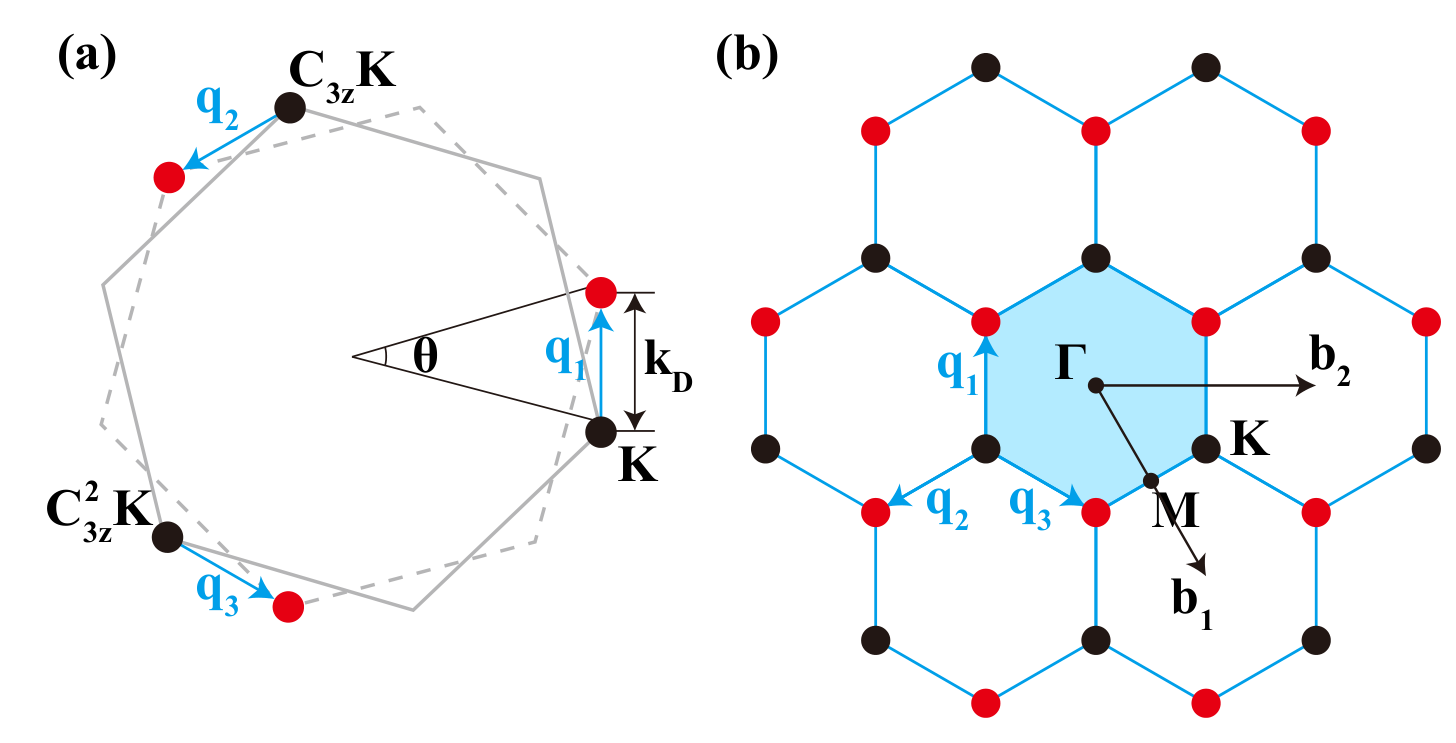
\includegraphics[width=0.8\linewidth]{fig/moire-vectors.png}
\end{figure}

\n

This \textbf{BM model} is called \textbf{MBM-1V (Moiré Band Model - One Valley)} by Bernevig. If we decompose $\q = \k - \Q$, $\q'=\k-\Q'$, where $\Q$ and $\Q'$ belong to the hexagonal lattice formed by adding $\q_{1,2,3}$ iteratively, we can rewrite the hamiltonian as
$$
\boxed{
H_{\Q, \Q'}^{(\text{MBM-1V})}(\k) =
\delta_{\Q,\Q'} v_F (\k-\Q) \vdot \bm{\sigma}
+ w \sum_{j=1}^{3} (\delta_{\Q'-\Q, \q_j} + \delta_{\Q-\Q', \q_j}) T^j.
}
$$

\begin{itemize}
\item This model is \textbf{topological} and is what we have been discussing the whole time.
\item The tables of Bernevig apply to this model, where we consider the Wyckoff position 1a within the THF approach to solve the topological obstruction.
\item Its magnetic space group is $P6'2'2$. Generators: $C_{6z} T$, $C_{2y} T$, $C_{2x}$.
\end{itemize}

\begin{table}[H]
\scriptsize
\caption{Elementary band representations of the magnetic space group $P6'2'2$.}
\centering
\begin{tabular}{|c|c|c|c|c|c|c|c|c|}
\hline
Wyckoff & \multicolumn{3}{c|}{$1a$} & \multicolumn{3}{c|}{$2c$} & \multicolumn{2}{c|}{$3f$} \\
\cline{1-9}
Site sym. & \multicolumn{3}{c|}{$6'2'2$, $32$} & \multicolumn{3}{c|}{$32$, $32$} & \multicolumn{2}{c|}{$2'2'2$, $2$} \\
\cline{1-9}
EBR & $G_{A_1}^{1a}(1)$ & $G_{A_2}^{1a}(1)$ & $G_{E}^{1a}(2)$ & $G_{A_1}^{2c}(2)$ & $G_{A_2}^{2c}(2)$ & $G_{E}^{2c}(4)$   & $G_{A}^{3f}(3)$ & $G_{B}^{3f}(3)$ \\
\hline
$\Gamma$ & $\Gamma_1(1)$ & $\Gamma_2(1)$ & $\Gamma_3(1)$ & $2\Gamma_1(1)$ & $2\Gamma_2(1)$ & $2\Gamma_3(2)$ & $\Gamma_1(1)+\Gamma_3(2)$ & $\Gamma_2(1)+\Gamma_3(2)$ \\
\hline
$K$ & $K_1(1)$ & $K_1(1)$ & $K_2 K_3(2)$ & $K_2 K_3(2)$ & $K_2 K_3(2)$ & $2K_1(1) + K_2 K_3(2)$ & $K_1(1)+K_2 K_3(2)$ & $K_1(1)+K_2 K_3(2)$ \\
\hline
$M$ & $M_1(1)$ & $M_2(1)$ & $M_1(1)+M_2(1)$ & $2M_1(1)$ & $2M_2(1)$ & $2M_1(1)+2M_2(1)$ & $2M_1(1)+M_2(1)$ & $M_1(1)+2M_2(2)$ \\
\hline
\end{tabular}
\label{tab:ebr-P6'2'2}
\end{table}

\begin{table}[H]
\caption{Character table of irreps at high symmetry momenta in magnetic space group $P6'2'2$.}
\centering
\begin{tabular} { c c c c | c c c | c c c }
\cline{1-10}
$\P$ & $\P \Gamma_1$ & $\P \Gamma_2$ & $\P \Gamma_3$ & $\P$ & $\P M_1$ & $\P M_2$ & $\P$ & $\P K_1$ & $\P K_2K_3$ \\
\cline{1-10}
$E$ & $\P1$ & $\P1$ & $\P2$ & $\P E$ & $\P1$ & $\P1$ & $\P E$ & $\P1$ & $\P2$ \\
$2 C_3$ & $\P1$ & $\P1$ & $ -1$ & $\P C_2'$ & $\P1$ & $ -1$ & $\P C_3$ & $\P1$ & $ -1$ \\
$3 C_2'$ & $\P1$ & $ -1$ & $\P0$ & $\P$ & $\P$ & $\P$ & $\P C_3^{-1}$ & $\P1$ & $-1$ \\
\cline{1-10}
\end{tabular}
\label{tab:char-P6'2'2}
\end{table}

%%%%%%%%%%%%%%%%%%%%%%%%%%%%%%%%%%%%%%%%%%%%%%%%%%%%%%%%%%%%%%%%%%%%%%%%%%%%%%%%%%%%%%%%%%%%%%%%%%
\section{There exists another model}
%%%%%%%%%%%%%%%%%%%%%%%%%%%%%%%%%%%%%%%%%%%%%%%%%%%%%%%%%%%%%%%%%%%%%%%%%%%%%%%%%%%%%%%%%%%%%%%%%%

According to Bernevig: ``The MBM-1V is half of the TBG system, with similar physics taking place in the electron states around $\K'$''. A model with the two valleys can be written as
$$
\boxed{
H_{\Q, \Q'}^{(\text{MBM-2V})}(\k) =
\delta_{\Q,\Q'} v_F (\k-\Q) \vdot \bm{\sigma} \otimes \tau_z
+ w \sum_{j=1}^{3} (\delta_{\Q'-\Q, \q_j} + \delta_{\Q-\Q', \q_j}) T^j \otimes \tau_0.
}
$$

Here $\tau_z$ and $\tau_0$ are the Pauli and identity matrix representing the valley degree of freedom.

\begin{itemize}
\item This model is \textbf{apparently different} from the latter, and \textbf{is not topological}. You can decompose it in EBR's as $G_{A_1}^{2c} + G_{A_2}^{2c}$.
\item The tables of Rennella apply to this model. There the authors (Vafek, Rennella, Angeli, Koshino, etc) consider Wyckoff position 2c, because these positions really correspond to symmetry-adapted exponentially localized Wannier functions.
\item The magnetic space group is $P6221'$. Generators: $C_{6z}$, $C_{2y}$, $C_{2x}$, $T$.
\end{itemize}

\begin{table}[H]
\caption{Elementary band representations generated from Wyckoff position $2c$ of the space group $P622$.}
\centering
\begin{tabular}{|c|c|c|c|}
\hline
Wyckoff & \multicolumn{3}{c|}{$2c$} \\
\cline{1-4}
Site sym. & \multicolumn{3}{c|}{$32$} \\
\cline{1-4}
EBR & $G_{A_1}^{2c}(2)$ & $G_{A_2}^{2c}(2)$ & $G_{E}^{2c}(4)$  \\
\hline
$\Gamma$ & $\Gamma_1(1) + \Gamma_4(1)$ & $\Gamma_2(1) + \Gamma_3(1)$ & $\Gamma_5(2) + \Gamma_6(2)$ \\
\hline
$K$ & $K_3(2)$ & $K_3(2)$ & $K_1(1) + K_2(1) + K_3(2)$ \\
\hline
$M$ & $M_1(1) + M_4(1)$ & $M_2(1) + M_3(1)$ & $M_1(1) + M_2(1) + M_3(1) + M_4(1)$ \\
\hline
\end{tabular}
\label{tab:ebr-P622}
\end{table}

\begin{table}[H]
\caption{Character table of irreps at high symmetry momenta in space group $P622$.}
\scriptsize
\centering
\begin{tabular} { c c c c c c c | c c c c c | c c c c }
\cline{1-16}
$\P$ & $\P \Gamma_1$ & $\P \Gamma_2$ & $\P \Gamma_3$ & $\P \Gamma_4$ & $\P \Gamma_5$ & $\P \Gamma_6$ & $\P$ & $\P M_1$ & $\P M_2$ & $\P M_3$ & $\P M_4$ & $\P$ & $\P K_1$ & $\P K_2$ & $\P K_3$\\
\cline{1-16}
$E$      & $\P1$ & $\P1$ & $\P1$ & $\P1$ & $\P2$ & $\P2$ & $E$     & $\P1$ & $\P1$  & $\P1$ & $\P1$ & $E$      & $\P1$ & $\P1$ & $\P2$ \\
$2C_6$   & $\P1$ & $\P1$ & $ -1$ & $ -1$ & $ -1$ & $\P1$ & $C_2$   & $\P1$ & $\P1$  & $ -1$ & $ -1$ & $C_3$    & $\P1$ & $\P1$ & $ -1$ \\
$2C_3$   & $\P1$ & $\P1$ & $\P1$ & $\P1$ & $ -1$ & $ -1$ & $C_2'$  & $\P1$ & $ -1$  & $ -1$ & $\P1$ & $3C_2''$ & $\P1$ & $ -1$ & $\P0$ \\
$C_2$    & $\P1$ & $\P1$ & $ -1$ & $ -1$ & $\P2$ & $ -2$ & $C_2''$ & $\P1$ & $ -1$  & $\P1$ & $ -1$ &          &       &       &       \\
$3C_2'$  & $\P1$ & $ -1$ & $ -1$ & $\P1$ & $\P0$ & $\P0$ &         &       &        &       &       &          &       &       &       \\
$3C_2''$ & $\P1$ & $ -1$ & $\P1$ & $ -1$ & $\P0$ & $\P0$ &         &       &        &       &       &          &       &       &       \\
\cline{1-16}
\end{tabular}
\label{tab:char-P622}
\end{table}

Compare tables \ref{tab:ebr-P622} and \ref{tab:char-P622} with tables 2.5 and (2.1, 2.3) of Rennella \cite{thesis_rennella}, respectively.

%%%%%%%%%%%%%%%%%%%%%%%%%%%%%%%%%%%%%%%%%%%%%%%%%%%%%%%%%%%%%%%%%%%%%%%%%%%%%%%%%%%%%%%%%%%%%%%%%%
\section{Numerical Results}
%%%%%%%%%%%%%%%%%%%%%%%%%%%%%%%%%%%%%%%%%%%%%%%%%%%%%%%%%%%%%%%%%%%%%%%%%%%%%%%%%%%%%%%%%%%%%%%%%%

\begin{figure}[H]
\centering
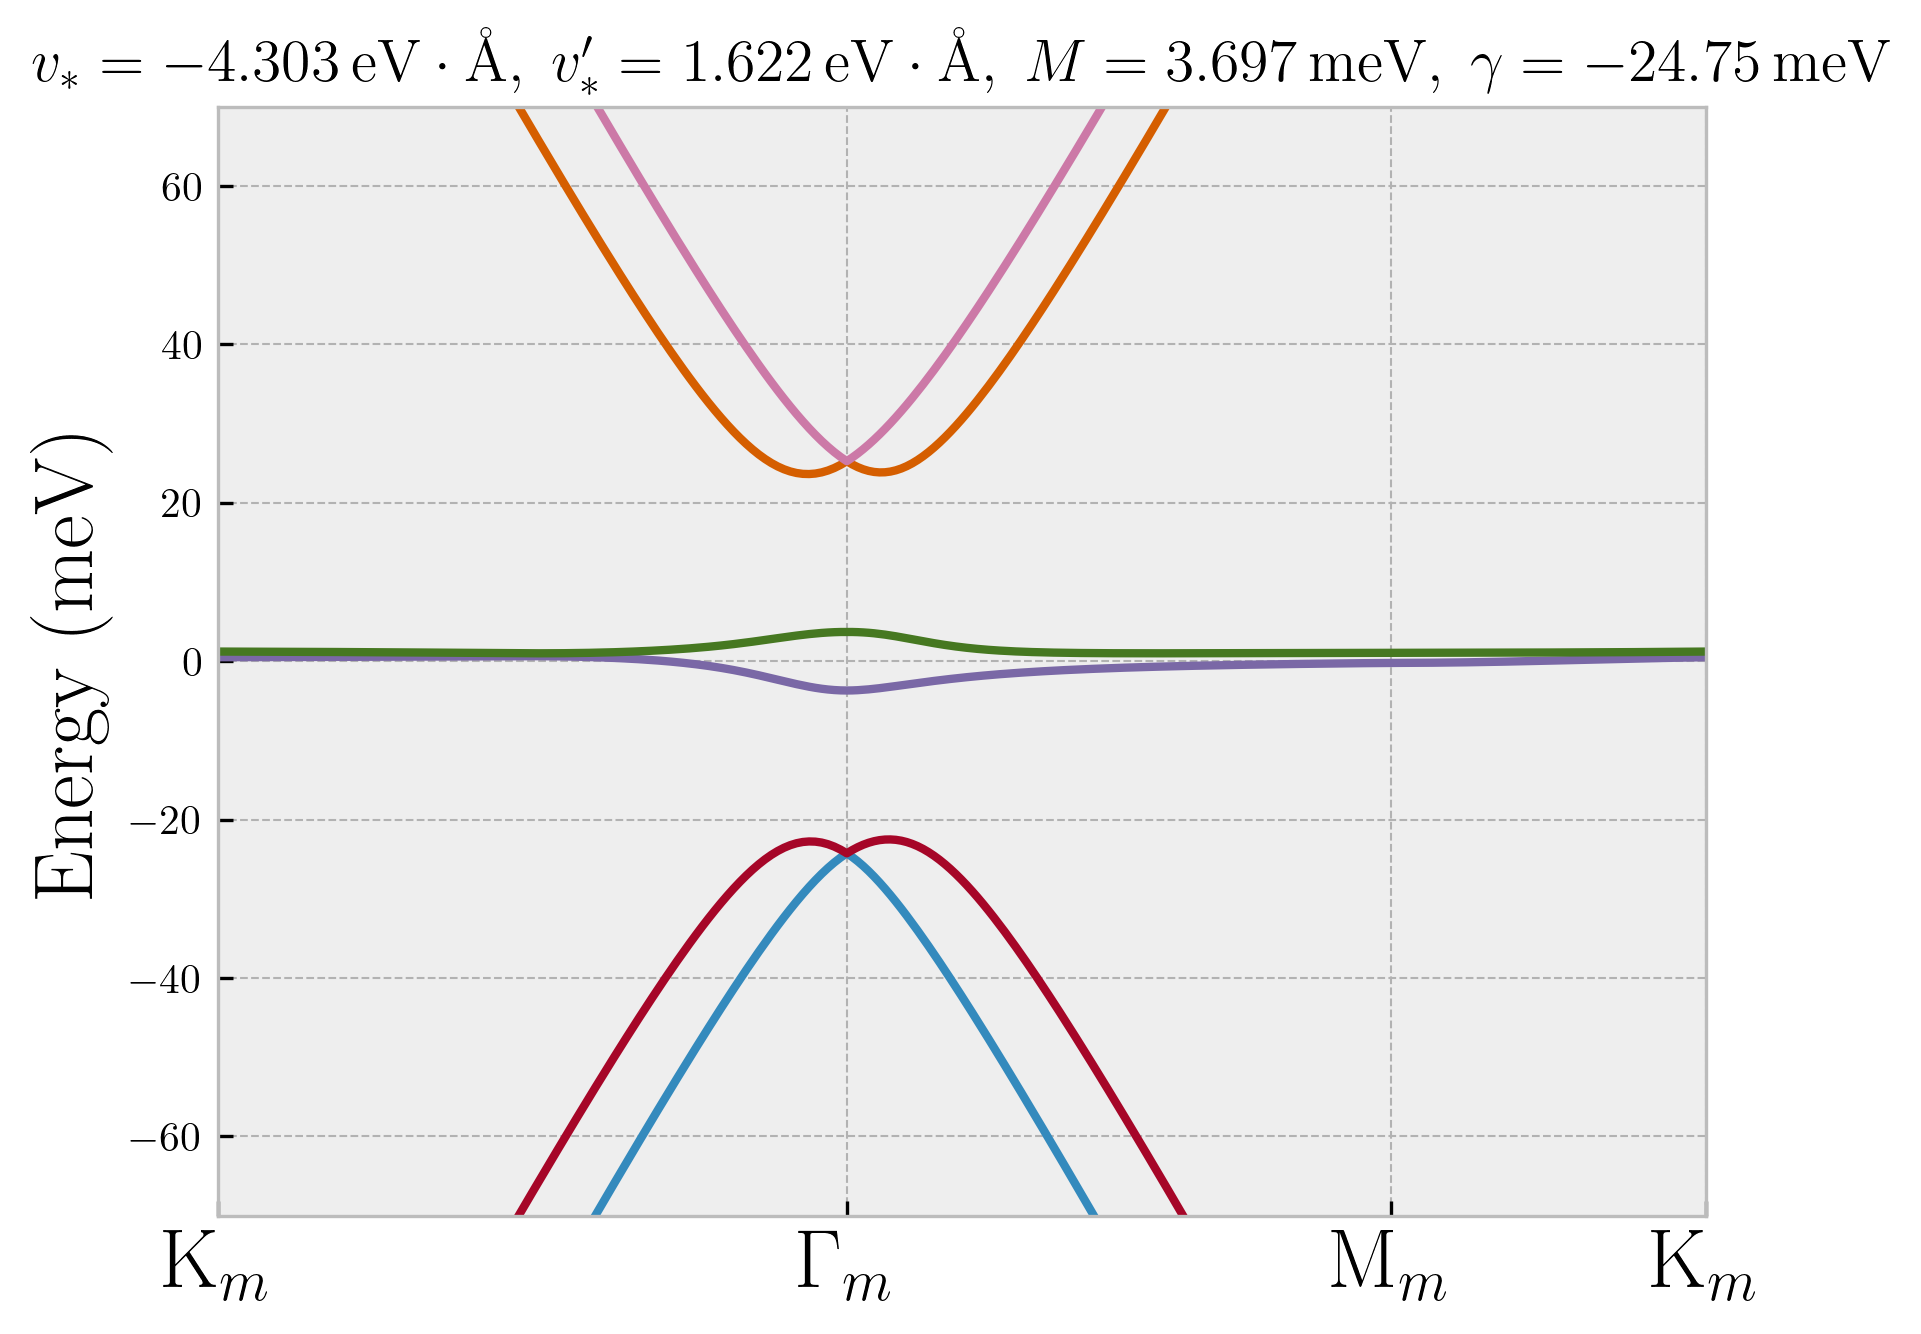
\includegraphics[height=0.35\linewidth]{fig/thf-correct_params.png}
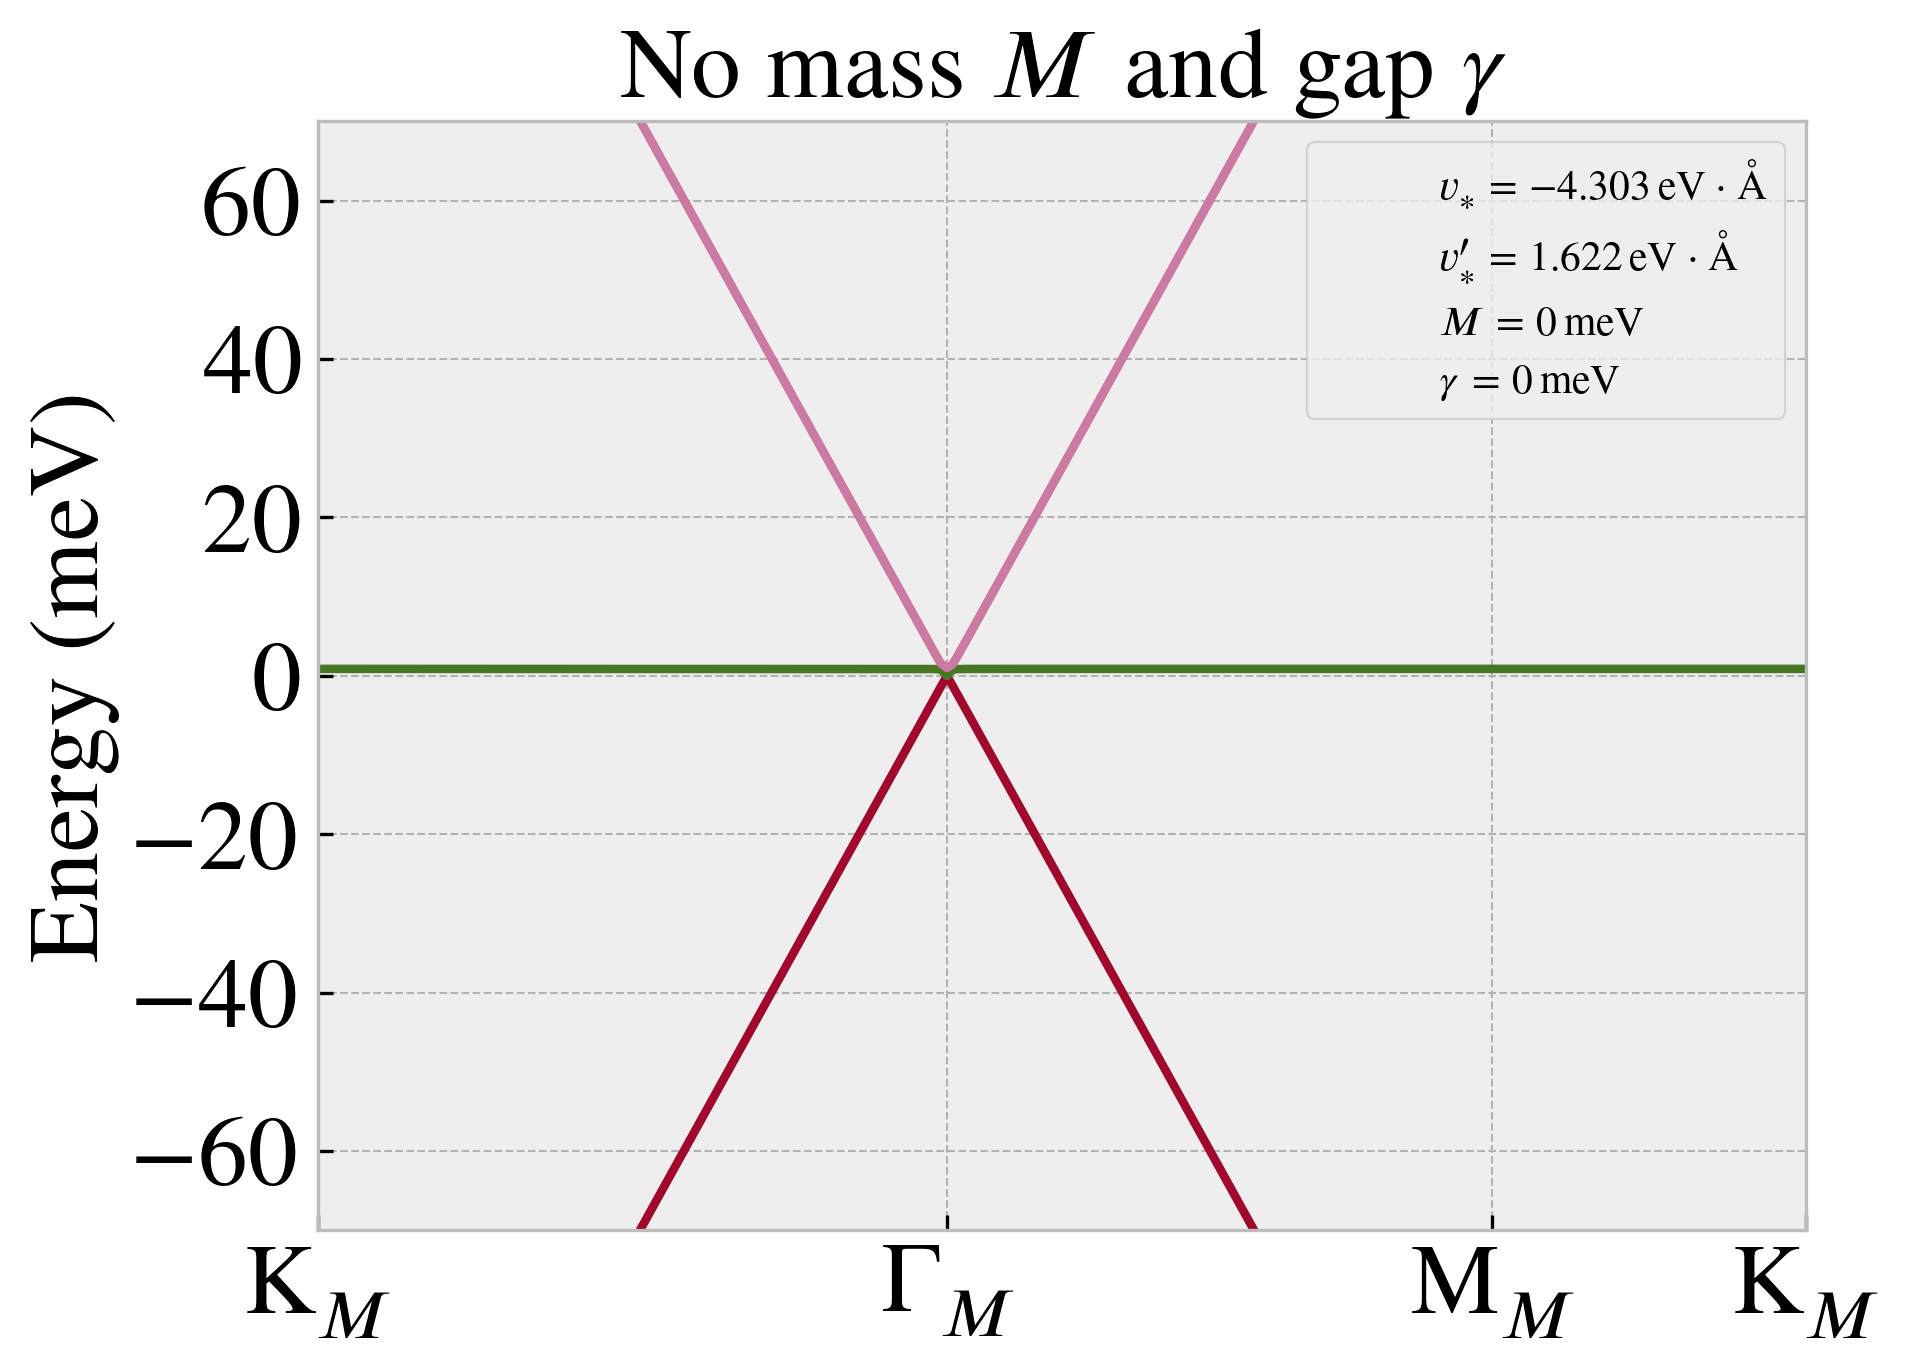
\includegraphics[height=0.35\linewidth]{fig/thf-no_M_no_gamma.png}
%\caption{}
\label{fig:thf-correct_params}
\end{figure}

\begin{figure}[H]
\centering
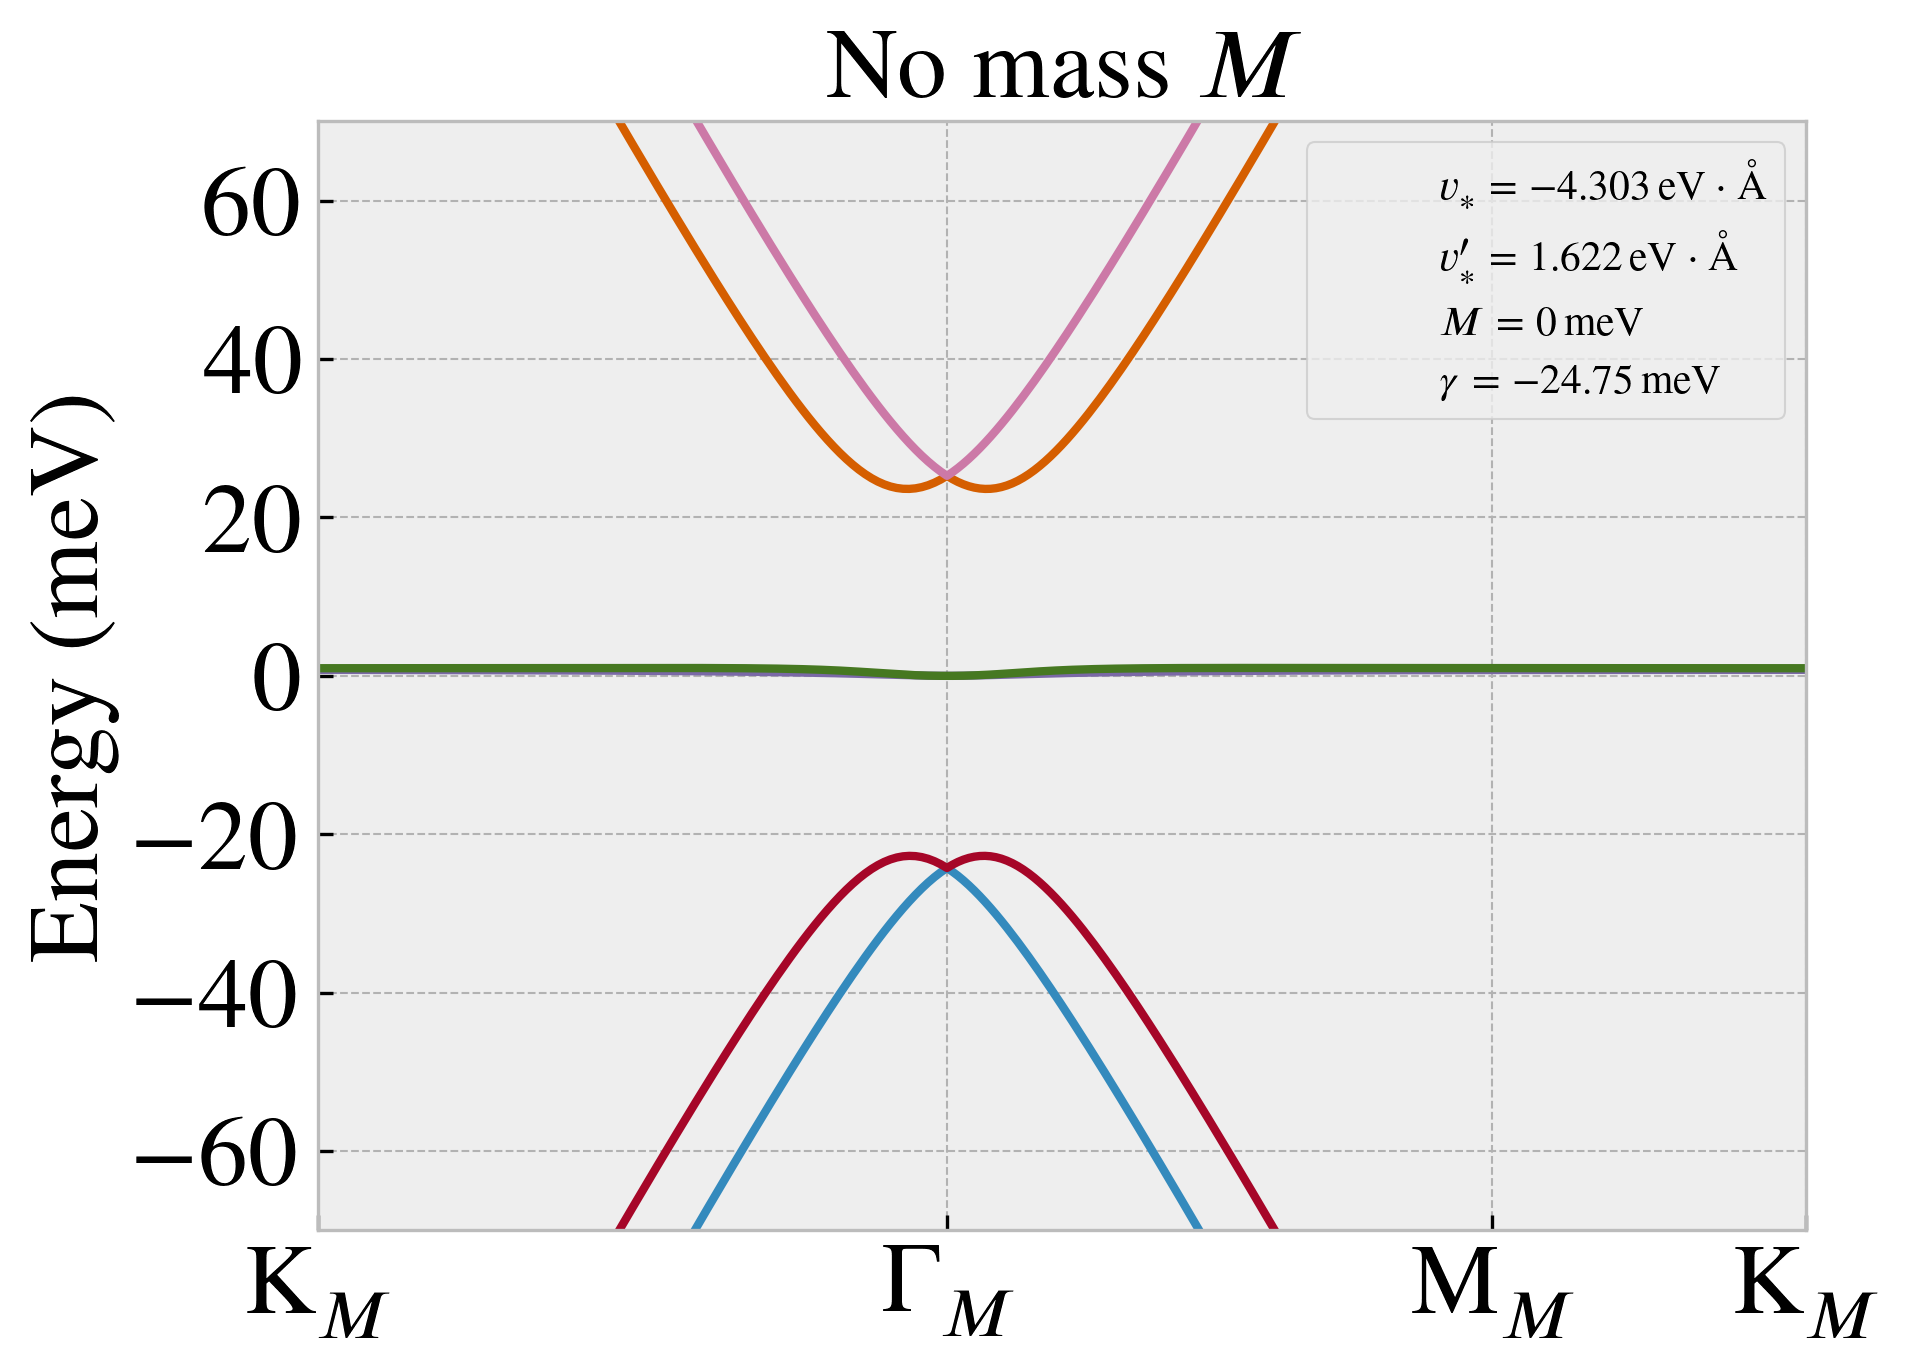
\includegraphics[height=0.35\linewidth]{fig/thf-no_M.png}
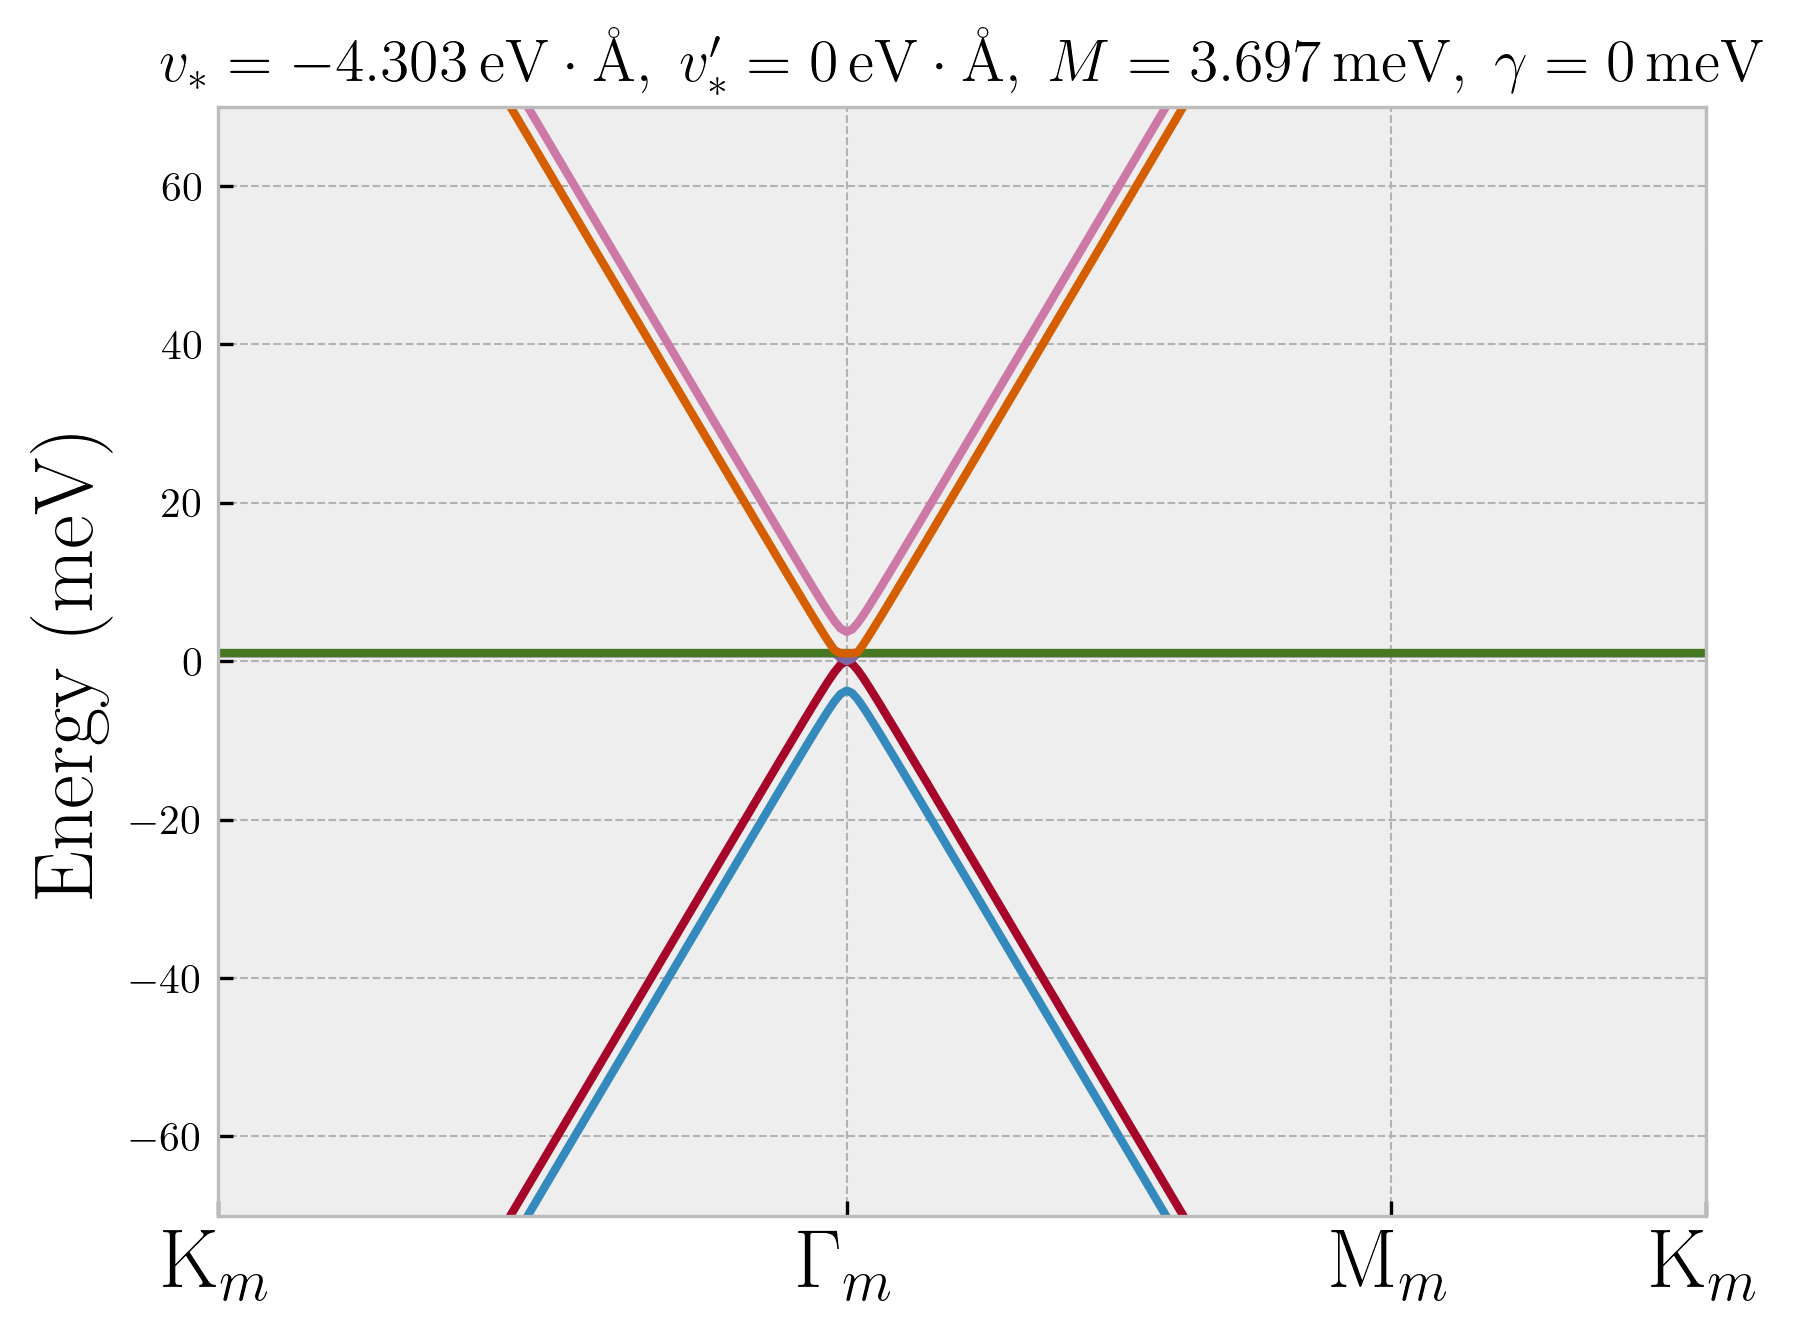
\includegraphics[height=0.35\linewidth]{fig/thf-no_coupling.png}
%\caption{}
\label{fig:thf-exploration}
\end{figure}



%%%%%%%%%%%%%%%%%%%%%%%%%%%%%%%%%%%%%%%%%%%%%%%%%%%%%%%%%%%%%%%%%%%%%%%%%%%%%%%%%%%%%%%%%%%%%%%%%%
%%%%%%%%%%%%%%%%%%%%%%%%%%%%%%%%%%%%%%%%%%%%%%%%%%%%%%%%%%%%%%%%%%%%%%%%%%%%%%%%%%%%%%%%%%%%%%%%%%


%%%%%%%%%%%%%%%%%%%%%%%%%%%%%%% COMMENT THIS TO COMPILE main.tex %%%%%%%%%%%%%%%%%%%%%%%%%%%%%%%%
%%-----
%% Referências bibliográficas
%%-----
\addcontentsline{toc}{chapter}{\bibname}
%\bibliographystyle{abntex2-num}
\bibliography{citations}
\bibliographystyle{ieeetr}
\end{document}
%%%%%%%%%%%%%%%%%%%%%%%%%%%%%%% COMMENT THIS TO COMPILE main.tex %%%%%%%%%%%%%%%%%%%%%%%%%%%%%%%%
